\documentclass{article}

\PassOptionsToPackage{numbers,compress}{natbib}
\usepackage[dblblindworkshop]{neurips_2026}
\workshoptitle{Physical Understanding for Decision-Making: Bridging Foundation Models and Reliable Agents}

\usepackage[utf8]{inputenc}
\usepackage[T1]{fontenc}
\usepackage{courier}
\usepackage[hidelinks,hypertexnames=false]{hyperref}
\usepackage{url}
\usepackage{booktabs}
\usepackage{amsmath}
\usepackage{amsfonts}
\usepackage{graphicx}
\usepackage{float}
\usepackage{microtype}
\usepackage{xcolor}
\usepackage{placeins}
\usepackage{adjustbox}


\newcommand{\method}{SafeVantage}
\newcommand{\hmthree}{HM3D-Sem}
\newcommand{\support}{\mathrm{support}}

\title{\method: Vantage-Aware Memory for Reliable Embodied Decisions}

\author{Sean Hardesty Lewis$^{1}$ \and Zuyi Guo$^{2}$ \and Benwang Chen$^{2}$ \and Zirui Li$^{3}$ \and Hongyi Lin$^{4}$ \and Heye Huang$^{*2}$\\[2pt]
Massachusetts Institute of Technology, Cambridge, MA, USA$^{1}$\\
Cho Chun Shik Graduate School of Mobility, KAIST, Daejeon, South Korea$^{2}$\\
School of Mechanical and Aerospace Engineering, Nanyang Technological University, Singapore$^{3}$\\
School of Vehicle and Mobility, Tsinghua University, Beijing, China$^{4}$}

\begin{document}

\maketitle

\begin{abstract}
Embodied agents must decide both \emph{where to look} and \emph{when the evidence warrants a decision}. We present \method{}, a semantic memory and active-perception policy that records the views supporting each claim. The policy uses this evidence state to select corroborating views and to output \textsc{Yes}, \textsc{No}, or \textsc{Wait}. On a held-out ProcTHOR test spanning 232 unseen houses and 7,424 paired episodes per method and action budget, \method{} raises macro-F1 from 0.4845 to 0.5289 and reduces travel from 7.23 to 3.56~m at eight actions, while risk falls from 0.3964 to 0.3872. The same pattern holds at twelve actions: macro-F1 rises from 0.5855 to 0.6270, risk falls from 0.3685 to 0.3523, and travel falls from 8.42 to 7.90~m. On a separate 96-house cohort, removing supporting-view identity, target-ray alignment, and yaw diversity lowers macro-F1 by 4.35 points at eight actions and 1.15 at twelve. Equal-input HM3D comparisons show lower selective risk, and ScanNet interventions show that answer quality decreases when supporting views are removed and recovers when they are restored. Together, the results support vantage-aware memory as a useful interface between active perception and selective decision-making.
\end{abstract}

\begin{figure}[t]
  \centering
  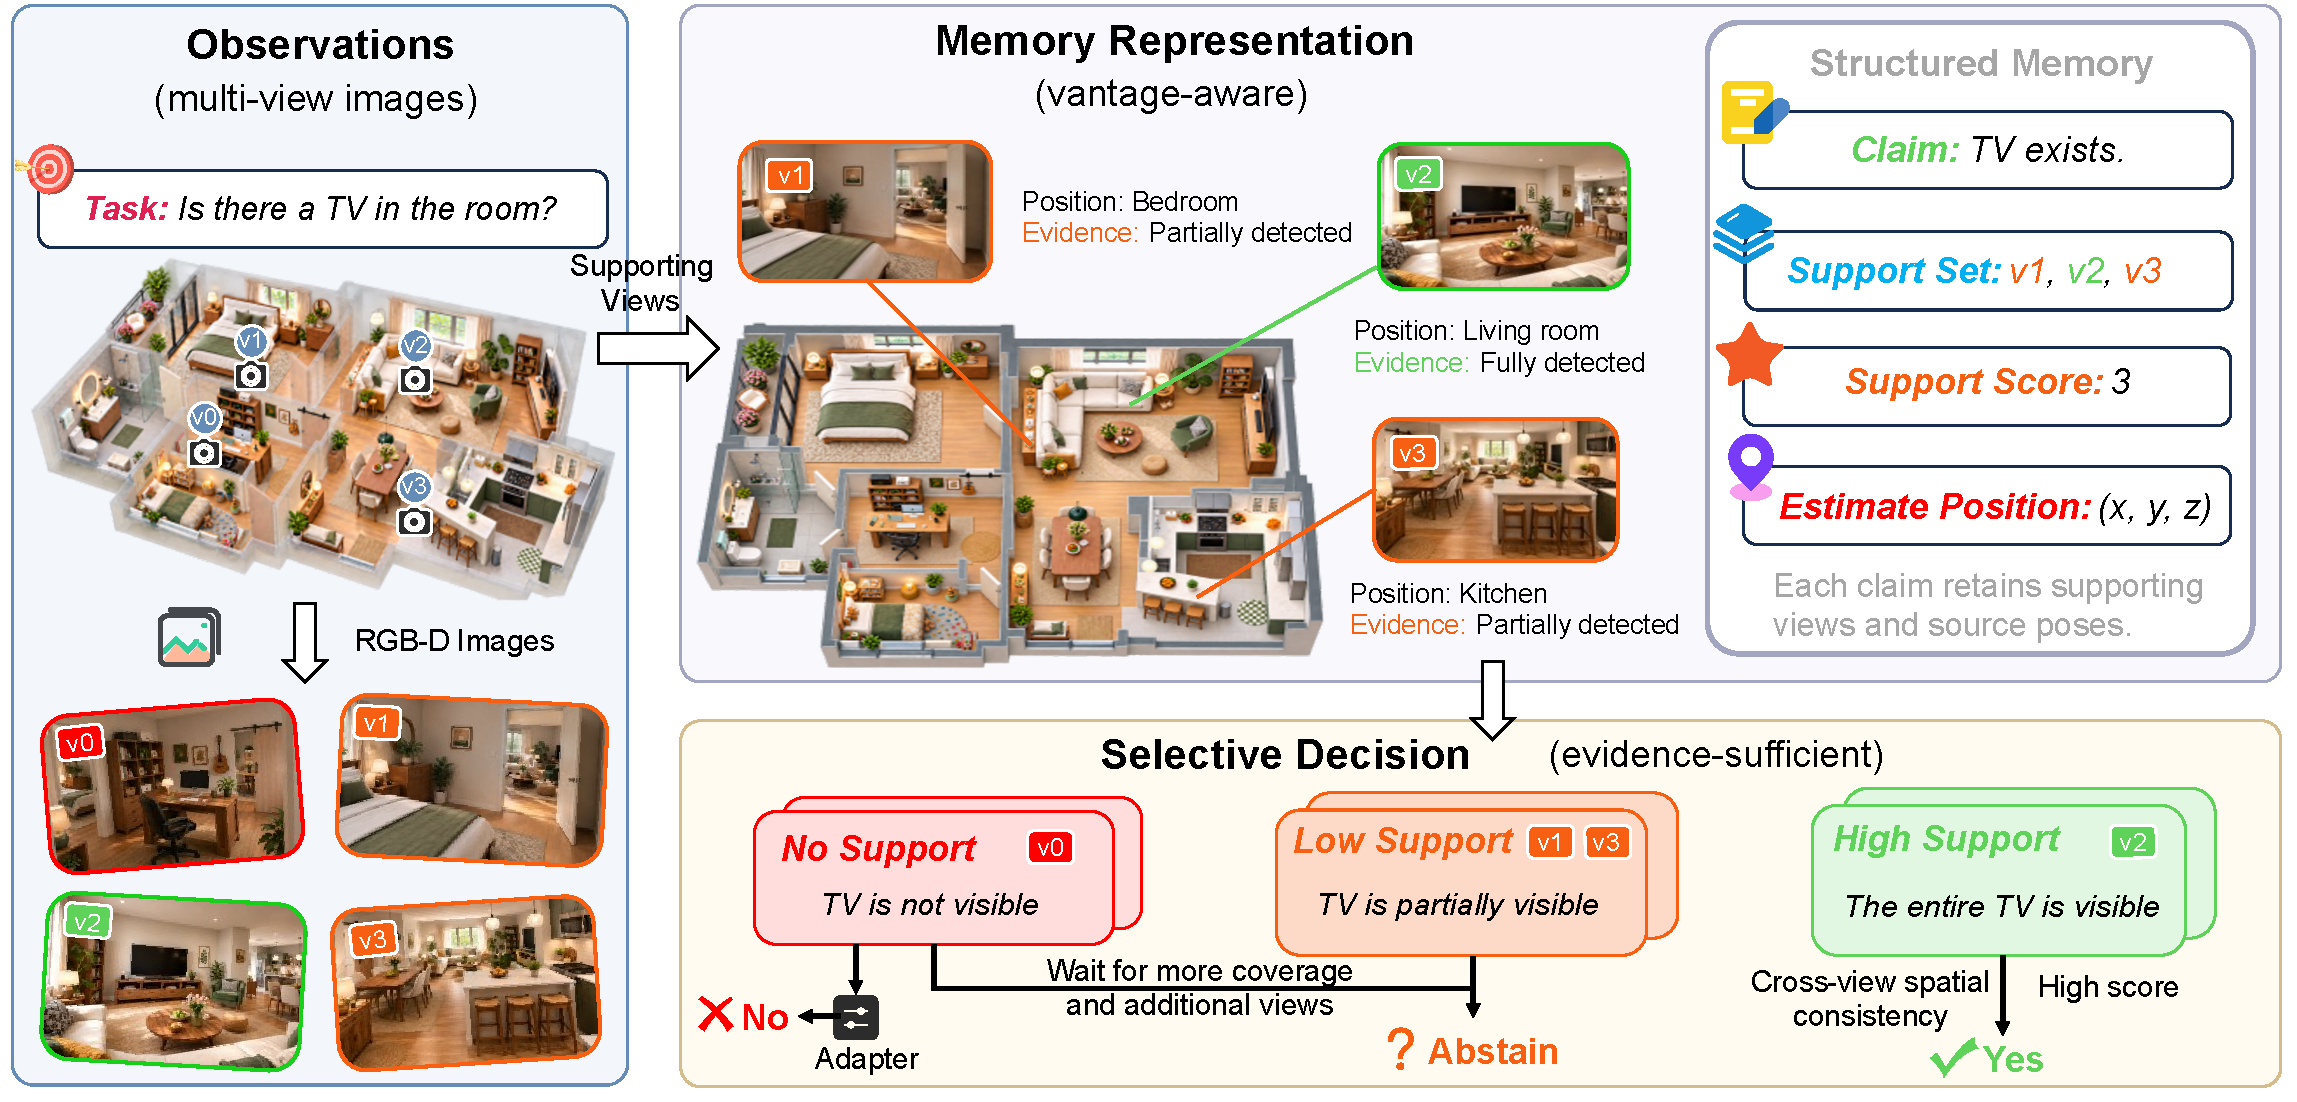
\includegraphics[width=\linewidth]{figures/zuyi_figure/framework_v2.pdf}
  \caption{\textbf{Overview of \method{}.} A vantage-aware memory retains the viewpoints supporting each claim and uses the evidence to select the next view and make the final \textsc{Yes}/\textsc{No}/\textsc{Abstain} decision.}
  \label{fig:teaser}
\end{figure}

\section{Introduction}
Recent advances in embodied AI connect language with spatial representations, persistent scene memory, and open-vocabulary questions about the physical world. OpenScene, VLMaps, and ConceptGraphs provide strong semantic interfaces for scene understanding and navigation~\citep{peng2023openscene,huang2023vlmaps,gu2024conceptgraphs}; EQA has progressed from active visual question answering to foundation-model benchmarks and confidence-guided exploration~\citep{das2018embodied,majumdar2024openeqa,exploreeqa2024}. Reliable embodied decisions, however, require more than retrieving a plausible semantic match: an agent must determine whether its observations provide sufficient evidence for the claim.

This requirement is especially important under partial observability. A map, stored image, or caption can retrieve a concept that was only weakly observed; conversely, a missing detection may only mean that no informative viewpoint was reached. Existing systems fuse visual-language features into maps, associate observations into object-centric graphs, or retain informative snapshots~\citep{huang2023vlmaps,gu2024conceptgraphs,yang2024threedmem}. These representations support retrieval and reasoning, but do not generally expose claim-level source-view support as a first-class signal for both selective decisions and the next observation.

We present \method{}, a \emph{vantage-aware} memory that associates each semantic claim with its supporting views, estimated target location, and missing evidence. Before detecting a target, the policy explores low-cost novel positions or category-relevant rooms. After a provisional detection, it seeks a second view that should observe the same target from a different position. A selective head then emits \textsc{Yes}, \textsc{No}, or \textsc{Wait}. The policy uses the same evidence state to decide what to observe and whether the accumulated evidence supports a decision (Figure~\ref{fig:teaser}).

We evaluate this acquisition-to-decision policy on a benchmark built from official ProcTHOR-10K splits~\citep{deitke2022procthor}. Across 232 unseen houses and 7,424 paired episodes per method and budget, \method{} improves macro-F1 while reducing risk and travel against the strongest equal-budget baseline at both horizons. Equal-input HM3D experiments and ScanNet view-removal studies test the same idea outside ProcTHOR. Our contributions are:
\begin{itemize}
  \item a vantage-aware memory that records which views support a claim, where the target is estimated to be, and what evidence is still missing;
  \item a ProcTHOR semantic active-view benchmark and learned-perception policy evaluated against five equal-budget acquisition baselines; and
  \item ablations and cross-environment studies showing when vantage-aware memory improves acquisition and downstream decisions.
\end{itemize}

\section{Related Work}
\textbf{Open-vocabulary spatial memory.}
VLMaps, OpenScene, LERF, ConceptGraphs, and OpenVoxel connect visual-language information to 2D maps, dense 3D features, radiance fields, object graphs, or captioned voxel groups~\citep{huang2023vlmaps,peng2023openscene,kerr2023lerf,gu2024conceptgraphs,huang2026openvoxel}. FARM further stores relational object structure and viewpoint evidence for large-scale retrieval~\citep{he2026farm}. These systems make rich evidence retrievable; \method{} uses supporting views for both acquisition and selective decisions. ConceptGraphs and VLMaps instantiate the map-centric alternative in our equal-input comparison.

\textbf{Embodied memory, question answering, and exploration.}
OpenEQA formalizes modern episodic and active EQA, while Explore-EQA calibrates confidence to decide when exploration may stop~\citep{majumdar2024openeqa,exploreeqa2024}. MemoryEQA, GraphEQA, and 3D-Mem organize historical observations, scene graphs, and informative snapshots for retrieval and exploration~\citep{memoryeqa2025,saxena2025grapheqa,yang2024threedmem}. EXPRESS-Bench evaluates whether answers are grounded in exploration~\citep{jiang2025express}; Mind Palace studies long-term active EQA with value-of-information stopping~\citep{ginting2025mindpalace}. DAAAM and UQ-DAAAM extend memory to real-time 4D scene graphs and cross-view semantic uncertainty~\citep{gorlo2025daaam,zhang2026uqdaaam}. \method{} studies a complementary interface: how supporting views determine both the next observation and the final decision.

% \textbf{Decision-conditioned planning and interactive worlds.}
% VLM-TAMP uses VLM subgoals to guide feasibility-checked task-and-motion planning, while PIGINet ranks plan skeletons before expensive refinement~\citep{yang2024vlmtamp,yang2023piginet}. GeniWorld represents robot kinematics as spatially aligned visual actions for closed-loop predictive simulation~\citep{gu2026geniworld}. We share their emphasis on inspectable state, action, and consequence, but ask whether stored visual evidence supports a semantic decision. Our Habitat traces show this connection between action, observation, and decision.

\textbf{Selective prediction and abstention.}
Selective prediction studies the risk--coverage tradeoff created by a reject option~\citep{geifman2019selectivenet}. KnowNo applies conformal prediction to robot planners that ask for help under ambiguity~\citep{ren2023knowno}; Explore-EQA calibrates stopping during visual exploration~\citep{exploreeqa2024}. AbstainEQA shows that embodied agents still struggle to withhold answers when perceptual evidence is unavailable or underspecified~\citep{wu2026abstaineqa}. \method{} shares the abstention goal, but grounds it in viewpoint support within semantic memory.

\section{Method}
\subsection{Vantage-Aware Semantic Memory}
For each scene, \method{} captures a set of posed observations $o_i=(I_i,D_i,T_i,t_i)$ containing RGB, optional depth, camera pose, and time. A semantic claim $c$ is represented by a support set
\begin{equation}
  V(c) = \{v_i : c \text{ is detected from vantage } v_i\},
\end{equation}
and a support score
\begin{equation}
  \support(c) = |V(c)|.
\end{equation}
When depth and pose are available, support views also provide approximate 3D localization by back-projecting observed pixels. The core memory record is therefore not only concept identity, but the tuple
\begin{equation}
  m(c) = (c, V(c), \support(c), \hat{x}_c),
\end{equation}
where $\hat{x}_c$ is an optional 3D centroid estimate. ``Detected'' is adapter-specific: ProcTHOR uses YOLO-World scores and boxes~\citep{cheng2024yoloworld}, while the HM3D study uses Qwen2-VL-7B per-view object lists~\citep{wang2024qwen2vl}. Simulator semantics provide evaluation labels and exact-view diagnostics. Keeping support explicit lets a policy inspect which views justify a claim and distinguish one weak observation from a repeated spatial pattern.

\paragraph{Evidence semantics.}
Vantage-aware memory separates four quantities: \emph{target visibility},
whether the queried instance appears; \emph{property or relation sufficiency},
whether the view reveals the required attribute or configuration;
\emph{search coverage}, whether the relevant region has been observed well
enough to support a negative claim; and \emph{answer correctness}, which
also depends on the downstream reader. These quantities are related but not
equivalent: visibility may be insufficient for attributes or relations, and
a correct answer may occasionally arise without sufficient visual evidence.

Figure~\ref{fig:coverage} illustrates this distinction spatially.
Target-visible viewpoints provide positive support, whereas partial or
context-only observations remain unresolved. Therefore, missing support does
not by itself imply semantic absence; it may simply reflect incomplete
coverage. Sufficient direct evidence can support a positive commitment,
while partial or contextual evidence should favor deferment.
Our main task focuses on category presence, where repeated target support
provides positive evidence. An empty support set remains unresolved unless
the calibrated adapter assigns the low-score region to \textsc{No}.
This asymmetry is fundamental: a supporting view can establish existence,
whereas absence requires sufficient coverage of the relevant search space.
Accordingly, SafeVantage treats viewpoint support and search coverage as
complementary signals.



\subsection{Claim-Conditioned Active Acquisition}
Let $H_t$ be the posed observation history and $\mathcal{A}_t$ the unvisited viewpoints reachable within the remaining geodesic budget. Before a provisional target detection, \method{} balances spatial novelty, category--room evidence, and travel. After a detection, the evidence state supplies a provisional target ray and the locations of supporting views. A candidate receives value for aligning with that ray, viewing the estimated target location from a distinct position, staying near a useful triangulation baseline, and covering new space; travel enters as $(0.5+d(a))^{-p}$. In compact form,
\begin{equation}
 a_t^*=\arg\max_{a\in\mathcal{A}_t}
 \frac{G_{\mathrm{corr}}(a;H_t)+\lambda_r G_{\mathrm{ray}}(a;H_t)}{(0.5+d(a))^p}
 +\lambda_c G_{\mathrm{cov}}(a;H_t),
\end{equation}
where $G_{\mathrm{corr}}$ combines proximity to the current hypothesis with distinct-position and yaw diversity, and $G_{\mathrm{ray}}$ rewards cameras facing the score-weighted grounded target estimate. Candidate edges are capped locally after detection, preventing an uncertain hypothesis from inducing a long chase. The eight-action policy emphasizes low-cost novelty; the twelve-action policy allows broader coverage. Their parameters are selected on training and nested validation scenes and then held fixed.

The policy favors views that resolve uncertainty at low travel cost. Its exploration branch seeks an initial supporting view, and its corroboration branch tests the provisional detection from a second viewpoint. The selective head uses the resulting evidence state for the final decision.

All compared policies operate on the same action graph. Random chooses a deterministic hash-random candidate; nearest frontier minimizes incremental geodesic distance; coverage gain maximizes newly covered positions; category-room prior combines coverage with a training-derived room model; and detector-confidence gain seeks a distinct nearby view around the strongest detection. \method{} builds on detector-confidence gain by adding target-ray alignment, supporting-view diversity, and budget-conditioned exploration.

\begin{figure*}[t]
  \centering
  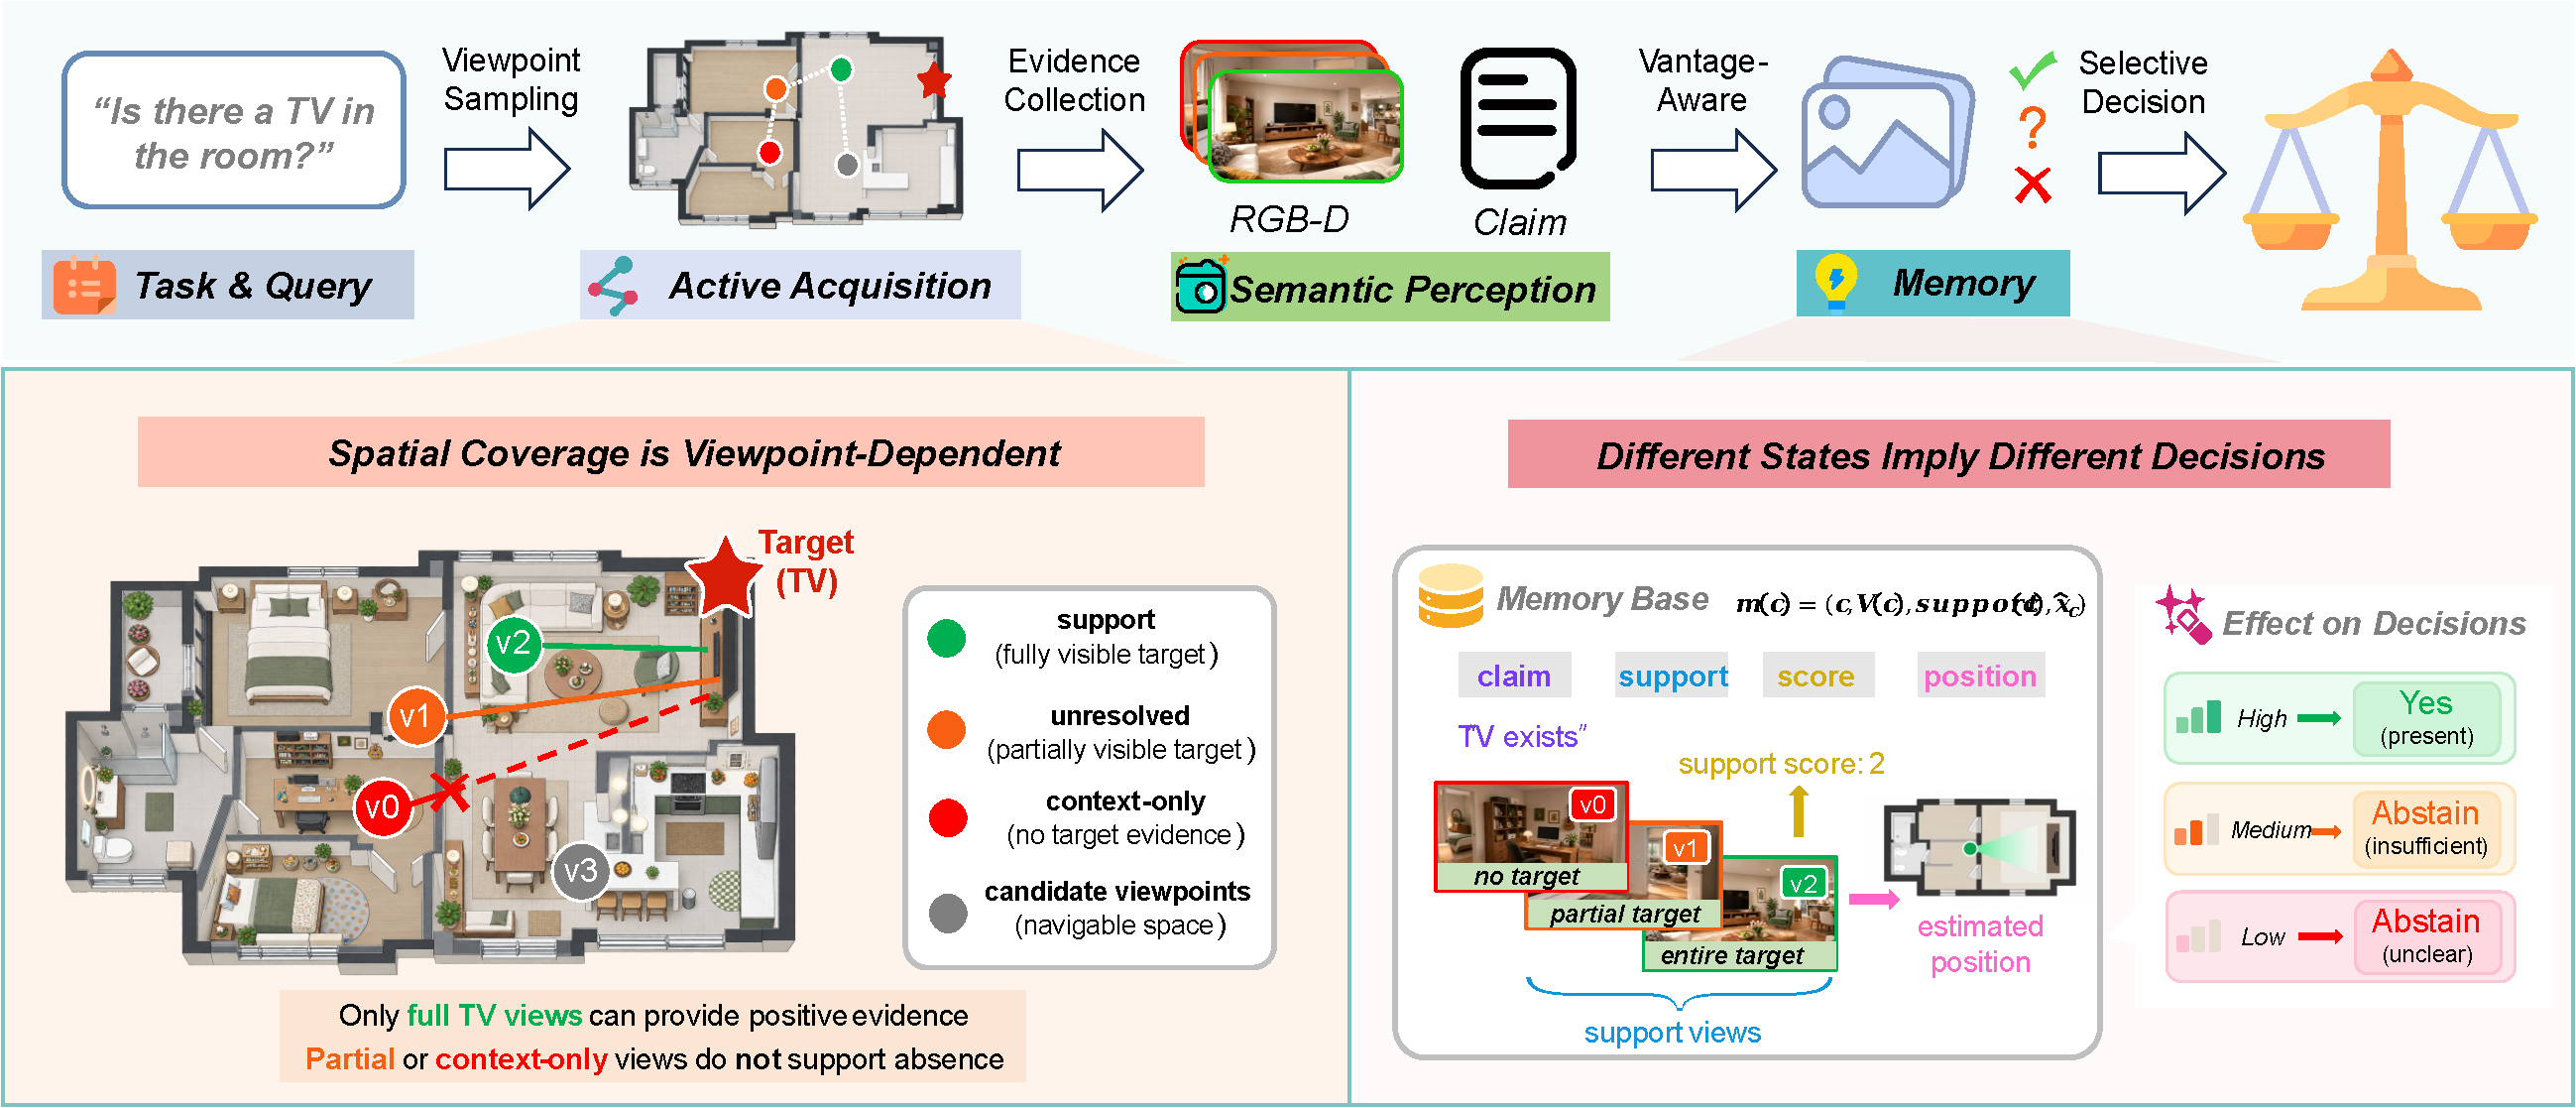
\includegraphics[width=0.96\textwidth]{figures/zuyi_figure/method.pdf}
  \caption{
  \textbf{Viewpoint support and search coverage provide complementary evidence.}
  Navigable viewpoints differ in the target evidence they reveal. Supporting
  observations provide positive evidence, whereas partial or context-only
  observations do not justify absence. Retained views and target geometry
  inform subsequent acquisition and selective decisions.
  }
  \label{fig:coverage}
\end{figure*}

\subsection{Acquisition-to-Decision Head}
After the fixed action horizon, a selective head summarizes the claim state using the top three scores from distinct positions, support counts at five thresholds, observed-position coverage, distinct rooms, observation count, grounded-evidence fraction, minimum inter-view target distance, maximum context evidence, and category identity. An $\ell_2$-regularized logistic model is fitted independently for each policy using five scene-disjoint training folds. A positive decision additionally requires a pair of distinct supporting positions whose grounded target estimates agree within a fixed radius. Thus
\begin{equation}
 \pi(H_T)=
 \begin{cases}
  \textsc{Yes}, & P(y{=}1\mid H_T)\geq\alpha \ \wedge\ \mathrm{pair}(H_T),\\
  \textsc{No}, & P(y{=}1\mid H_T)\leq\beta,\\
  \textsc{Wait}, & \text{otherwise.}
 \end{cases}
\end{equation}
The SafeVantage thresholds are selected by nested validation; every baseline head is fitted from training-only out-of-fold rows.

\subsection{Evidence-Sufficient Decisions}
The active ProcTHOR benchmark uses the policy-specific head above. For the static cross-environment comparisons, where each method exposes only a scalar score, we instead use the following shared two-threshold adapter:
\begin{equation}
\pi_{\tau_-,\tau_+}(c) =
\begin{cases}
\textsc{No}, & s(c) \le \tau_-,\\
\textsc{Abstain}, & \tau_- < s(c) < \tau_+,\\
\textsc{Yes}, & s(c) \ge \tau_+.
\end{cases}
\end{equation}
The thresholds are selected on calibration scenes and held fixed for evaluation. A method may decline to use the \textsc{No} branch when calibration does not justify it. Ties are broken toward higher coverage and then lower false-positive rate. The shared adapter measures how informative each memory score is under the same decision rule.

\subsection{Risk Objective}
We evaluate decisions with an asymmetric risk cost:
\begin{equation}
  R = 5\,\mathbb{1}[\mathrm{FP}] + 2\,\mathbb{1}[\mathrm{FN}] + 0.5\,\mathbb{1}[\mathrm{wait}] + 0.001\,C_\mathrm{resource}.
\end{equation}
False positives are weighted highest because unsupported positive decisions are the target failure mode in this setting. $C_\mathrm{resource}$ is geodesic travel in the active benchmark and view count in the static-memory protocol. We report macro-F1, answer rate, answered accuracy, false-positive rate on negative queries, resource use, and paired scene-bootstrap intervals alongside risk.

\subsection{Supporting-View Interventions}
Because every score is linked to source observations, we can remove and restore its visual evidence. For a question about a ScanNet instance, geometry identifies the target-visible ranks. We replace those ranks with target-absent frames while keeping history length and rank fixed, then restore the strongest one, the strongest four, or the complete target-view set. A reader-independent visibility test defines the intervention, and two VLM readers provide the outcomes. 


\section{Experimental Setup}
\textbf{ProcTHOR benchmark.}
Our primary evaluation uses official ProcTHOR-10K train, validation, and test identities~\citep{deitke2022procthor}. A 24-category vocabulary is derived from training metadata. Every scene contains 40 navigable positions with four camera yaws, yielding a common 160-view action graph with geodesic edge costs. The evaluator samples four present and four absent categories and four deterministic starts per category, producing 32 paired episodes per eligible scene. Policies receive RGB-D, pose, the training-derived vocabulary, and YOLO-World scores~\citep{cheng2024yoloworld}; object identity and hidden visibility are used only for evaluation.

\textbf{Test accounting.}
Of 256 held-out scene identities, 255 materialize successfully. The balanced-query rule yields 232 scenes and 7,424 paired episodes per method at each action budget; Appendix~\ref{app:contract} records the full protocol.

\textbf{Equal-budget policies.}
We evaluate random, nearest-frontier, coverage-gain, category--room-prior, detector-confidence-gain, and \method{} at horizons of eight and twelve actions under the same 20-m geodesic cap. All policies share the same scenes, starts, detector outputs, action budgets, feature schema, and decision-head architecture; all parameters are selected without test access. Five scene-disjoint folds fit a separate selective head for each policy. Nested validation selects the comparison policy at each budget: category--room prior at eight actions and detector-confidence gain at twelve.

Each acquisition variant and its training-fit selective head is also evaluated on 96 validation houses, yielding 3,072 paired episodes per variant and budget. A grouped intervention removes supporting-view identity, target-ray alignment, and yaw diversity together while preserving the remaining controller. A second contrast disables the pair gate in both policies to separate acquisition effects from decision-time consistency.

\textbf{Uncertainty and metrics.}
All comparisons are paired by scene, category, start, and budget. We report task risk, macro-F1 over positive and negative decisions, false-positive rate on absent queries, answer rate, accuracy conditional on answering, and mean geodesic travel. Confidence intervals use 10,000 paired bootstrap draws that resample whole scenes, preserving the 32 correlated episodes within each house.

\textbf{Complementary evidence studies.}
Thirty-six HM3D-Sem scenes~\citep{yadav2023hm3dsem} provide one common 160-view RGB-D/pose stream to \method{}, Qwen2 caption-RAG, ConceptGraphs, and released-code VLMaps. \method{} uses Qwen2-VL-7B object lists~\citep{wang2024qwen2vl}; Habitat semantics provide the query labels. A 41-concept vocabulary yields 1,436 presence queries, with nine disjoint calibration folds. A 73-question ScanNet intervention~\citep{dai2017scannet} removes and restores depth-verified views containing the queried instance. A 12-scene, 1,097-episode Habitat study~\citep{savva2019habitat} provides native 3D navigation traces in the appendix.

\section{Results}
\subsection{Held-Out Acquisition-to-Decision Performance}
Table~\ref{tab:locked-all-baselines} is the central result. It compares \method{} with five acquisition baselines at both action budgets using shared scenes, detectors, action graphs, and decision-head architecture.

\begin{table}[t]
\centering
\caption{
Equal-budget held-out ProcTHOR test.
\method{} ranks first in risk, macro-F1, and answer rate at both horizons;
bold marks each budget's best value. Travel is reported in meters.
}
\label{tab:locked-all-baselines}

\small
\renewcommand{\arraystretch}{1.10}
\setlength{\tabcolsep}{3.2pt}

\resizebox{0.98\columnwidth}{!}{%
\begin{tabular}{@{}clcccc@{}}
\toprule
Budget
& Method
& Risk$\downarrow$
& Macro-F1$\uparrow$
& Answer$\uparrow$
& Travel$\downarrow$ \\
\midrule

8
& \textbf{SafeVantage}
& \textbf{0.387}
& \textbf{0.529}
& \textbf{0.430}
& 3.56 \\

& Category-room prior
& 0.396
& 0.484
& 0.377
& 7.23 \\

& Nearest frontier
& 0.398
& 0.491
& 0.394
& \textbf{3.46} \\

& Detector-conf. gain
& 0.407
& 0.446
& 0.333
& 5.94 \\

& Coverage gain
& 0.422
& 0.406
& 0.305
& 6.31 \\

& Random
& 0.427
& 0.434
& 0.350
& 19.12 \\

\addlinespace[2pt]
\midrule

12
& \textbf{SafeVantage}
& \textbf{0.352}
& \textbf{0.627}
& \textbf{0.555}
& 7.90 \\

& Detector-conf. gain
& 0.369
& 0.585
& 0.516
& 8.42 \\

& Category-room prior
& 0.382
& 0.490
& 0.356
& 8.16 \\

& Coverage gain
& 0.385
& 0.534
& 0.471
& 8.97 \\

& Nearest frontier
& 0.395
& 0.464
& 0.337
& \textbf{5.28} \\

& Random
& 0.420
& 0.451
& 0.361
& 19.25 \\

\bottomrule
\end{tabular}%
}

\end{table}

At eight actions, the strongest validation-selected comparator is category--room prior. \method{} raises macro-F1 from 0.4845 to 0.5289 and answer rate from 0.3772 to 0.4296 while cutting travel from 7.23 to 3.56~m. Mean risk falls from 0.3964 to 0.3872; the paired difference is $-0.0091$ with 95\% CI $[-0.0174,-0.0008]$. SafeVantage therefore increases answer rate and macro-F1 while approximately halving travel. At twelve actions, the strongest comparator is detector-confidence gain. \method{} raises macro-F1 from 0.5855 to 0.6270, answer rate from 0.5163 to 0.5552, and answered accuracy from 0.8870 to 0.8945. It reduces travel from 8.42 to 7.90~m and risk from 0.3685 to 0.3523. The paired risk difference is $-0.0162$ ($[-0.0234,-0.0088]$), macro-F1 improves by 0.0415 ($[0.0336,0.0494]$), and travel falls by 0.52~m ($[-0.65,-0.39]$).



Figure~\ref{fig:locked-traces} follows one held-out positive query from route selection to decision. From the same start and eight-action budget, category--room prior travels 13.7~m without observing the paper towel and answers \textsc{No}; \method{} reaches the resolving view in 5.4~m and answers \textsc{Yes}.

\begin{figure}[t]
  \centering
  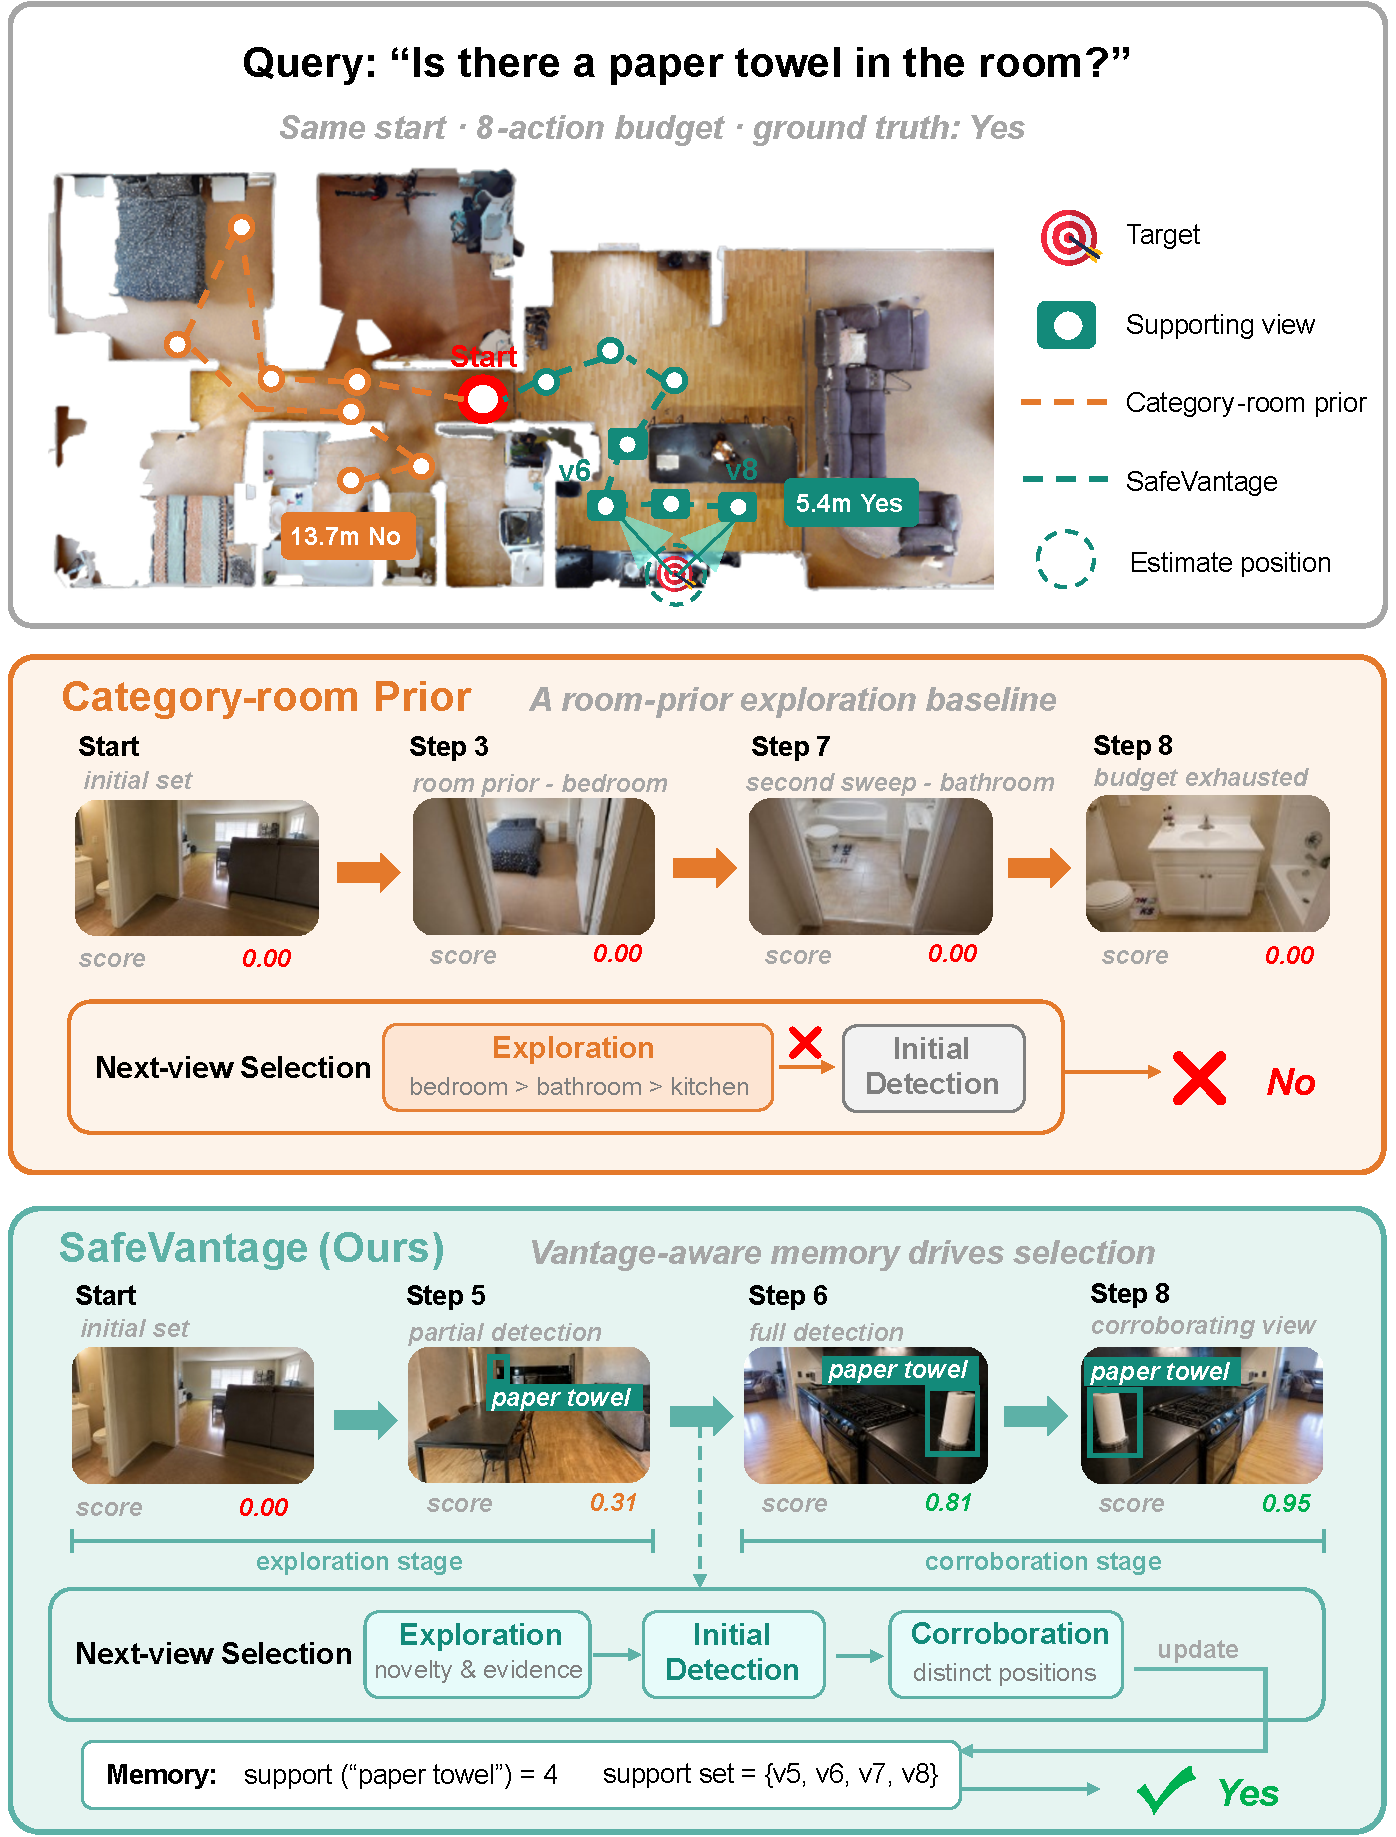
\includegraphics[width=\linewidth]{figures/zuyi_figure/example_v2.pdf}
  \caption{\textbf{One held-out episode for ``Is there a paper towel in the room?''} Both policies start from the same start with an 8-action budget and a positive ground-truth label. Category--room prior does not observe the target, answers \textsc{No}, and travels 13.7~m; \method{} acquires four supporting views, answers \textsc{Yes}, and travels 5.4~m.}
  \label{fig:locked-traces}
\end{figure}

\subsection{Supporting Views Drive the Policy}
To test the mechanism directly, we remove supporting-view identity, target-ray alignment, and yaw diversity together on a separate 96-house cohort. The detector, categories, starts, action horizons, room evidence, coverage features, geometry, and travel objective remain unchanged. Macro-F1 falls by 4.35 points at eight actions (95\% CI [3.23, 5.50]) and 1.15 points at twelve ([0.16, 2.16]). Figure~\ref{fig:grouped-vantage} also reports a contrast with the pair gate disabled in both policies, separating the acquisition effect from decision-time consistency.

\begin{figure}[t]
  \centering
  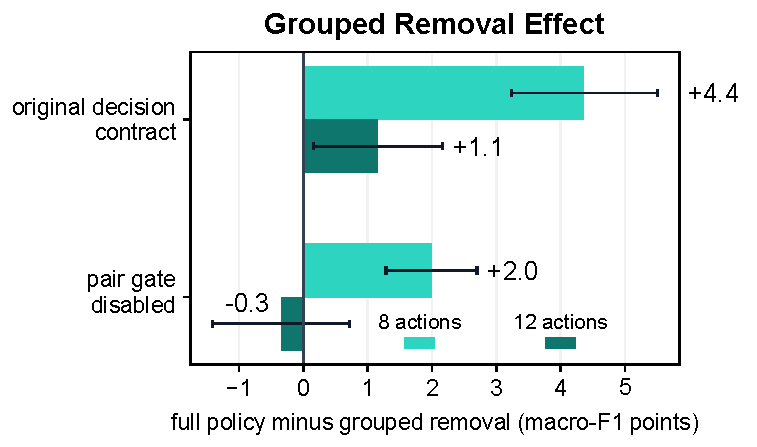
\includegraphics[
    width=\linewidth,
    height=0.25\textheight,
    keepaspectratio
  ]{figures/zuyi_figure/Fig_4.pdf}
  \caption{\textbf{Removing vantage-aware state lowers macro-F1.} Bars show full policy minus grouped removal on 96 validation houses; whiskers are paired 95\% intervals.}
  \label{fig:grouped-vantage}
\end{figure}

\subsection{Secondary Evidence in HM3D and ScanNet}
The ProcTHOR benchmark tests the complete active policy. We use HM3D and ScanNet as secondary tests of the underlying representation under fixed observations and controlled view removal.

Under an equal-input HM3D protocol, all methods receive the same 160 RGB-D/pose views. \method{} reaches risk 0.524, answered accuracy 0.962, and false-positive rate 0.059, compared with risk 0.617--0.715 for ConceptGraphs and caption-RAG and 0.618 for VLMaps. The ranking persists over nine disjoint calibration folds, matched coverage, and calibration-selected AURC; Appendix Table~\ref{tab:main} gives the complete comparison.

In the 73-question ScanNet intervention, removing all depth-verified views containing the queried instance lowers Qwen2-VL token F1 to 0.2483. Restoring four supporting views raises F1 to 0.4410, and restoring the complete set reaches 0.4540. The improvement from restoring the complete evidence set is positive for both Qwen2-VL and Qwen2.5-VL (Appendix Table~\ref{tab:causal}). Additional navigation and negative-decision diagnostics appear in Appendix~\ref{app:robustness}.

\section{Discussion}

SafeVantage shows that viewpoint provenance is useful not only for
remembering what has been observed, but also for deciding what evidence
should be acquired next. The ProcTHOR results indicate that retaining
supporting-view identity and target alignment improves equal-budget
acquisition and selective decisions, while the HM3D and ScanNet studies
show that the same representation remains informative under fixed
observations and controlled evidence removal. Together, these results
suggest that claim-level evidence can serve as a shared interface between
semantic memory, active perception, and selective decision-making.

The current study focuses on category-presence queries, discrete
viewpoint actions, and a fixed perception stack in simulated indoor
environments. Extending SafeVantage to attributes, relations, temporal
changes, continuous control, and real-robot settings will require more
general notions of evidence sufficiency and acquisition cost. These
directions provide a natural path toward question-conditioned and
coverage-aware embodied memory.


\section{Conclusion}

We presented SafeVantage, a vantage-aware semantic memory that retains
the viewpoints supporting each claim and uses the resulting evidence
state for both active acquisition and selective YES/NO/WAIT decisions.
On held-out ProcTHOR scenes, SafeVantage improves macro-F1 and reduces
decision risk relative to equal-budget acquisition baselines, while
requiring less travel than the strongest comparators. Component studies
further show that claim provenance, target-aware view selection, and
directed exploration contribute to these gains. Complementary HM3D and
ScanNet experiments support the same principle under fixed observations
and controlled evidence interventions, showing that viewpoint evidence
remains informative beyond the active acquisition setting. Overall, our
results suggest that embodied memory should retain not only what is
believed, but also which observations support the belief and what evidence
remains unresolved.

\textbf{Limitations.}
Our current evaluation focuses primarily on category-presence queries in
simulated indoor environments, using a fixed perception stack and a
discrete viewpoint action graph. These settings do not fully capture
detector shift, continuous control, or real-world sensing noise. In
addition, attributes, relations, temporal changes, and manipulation
preconditions may require richer notions of evidence sufficiency than
viewpoint support alone. Future work will extend SafeVantage toward
question-conditioned evidence acquisition, continuous control, and
real-robot evaluation.

\textbf{Societal Impact.}
SafeVantage aims to improve the reliability and auditability of embodied
agents by reducing unsupported semantic commitments and exposing the
visual evidence behind a decision. Potential applications include household
robots, inspection systems, and assistive agents. Practical deployment,
however, should account for sensor and environment shift, privacy of
captured observations, appropriate risk calibration, and safe fallback
behavior when evidence remains insufficient.

\setlength{\bibsep}{2pt plus 0.3ex}
\bibliographystyle{plainnat}
\bibliography{references}

\clearpage
\appendix

\section{Reproducibility and Experimental Protocol}
\label{app:contract}
\subsection{ProcTHOR Split and Frozen Evaluation}
\label{app:fresh-active}
The primary benchmark uses official ProcTHOR-10K splits, a training-derived 24-category vocabulary, 160 candidate viewpoints per scene, exact geodesic costs, and a 20-m travel cap. Of 256 held-out identities, 255 materialize; balanced-query construction yields 232 scenes and 7,424 paired episodes per method and action budget. Scene identities, detector predictions, action graphs, starts, queries, acquisition parameters, and decision heads are fixed before test evaluation. Policies never receive simulator instance identity or hidden visibility. The combiner requires identical $(\mathrm{scene},\mathrm{category},\mathrm{start},\mathrm{budget})$ keys and rejects duplicates before 10,000-draw paired whole-scene bootstrap analysis.

At eight actions, the frozen policy uses low-cost exploration, travel exponent 2.0, a 1.50-m edge cap, detection trigger 0.15, and ray weight 8.0; its positive/negative probabilities are 0.85/0.30 with support threshold 0.10 and 1.0-m pair radius. At twelve actions, it uses coverage exploration, exponent 3.0, a 0.75-m edge cap, trigger 0.10, and ray weight 2.0; the decision values are 0.40/0.30, support threshold 0.30, and the same pair radius. Both policies execute the complete horizon.

The comprehensive test adds training-only heads for random, nearest frontier, coverage gain, category--room prior, and detector-confidence gain while importing the byte-equivalent frozen \method{} model. It changes no scene, query, detector prediction, acquisition action, \method{} probability, or threshold.

The selected settings are Pareto-optimal in the 72-policy training archive. All six one-factor neighbors at each horizon retain joint improvements in risk, macro-F1, and travel.

\subsection{Complementary 3D Protocols}
The HM3D comparison fixes 36 scenes, a 41-concept vocabulary, and the same 160 RGB-D/pose observations per scene for every method. Its separate 1024-view semantic sweep is descriptive and excluded from scores. Each method exposes one scalar score per query and receives the same two-threshold adapter. Nine disjoint four-scene calibration folds evaluate the remaining 32 scenes. Qwen2-VL-7B captions all 5,760 frames for caption-RAG; ConceptGraphs and VLMaps use those same RGB-D/pose frames. An independent 8,628-row reconstruction verifies \method{} support counts and source-view identities.

For ScanNet, official instance geometry, camera pose, and depth determine whether the queried instance is visible. Target-visible frames are replaced at the same ranks by target-absent frames while history length, reader, prompt family, and question stay fixed. The complete condition restores the original supporting views; intervals cluster by scene. For the active HM3D diagnostic, 12 scene identifiers, 1,097 episodes, candidates, outputs, and two seeds are frozen. Candidates on disconnected navmesh islands are removed before scoring, and every displayed camera is an executed action from the metric candidate set.

\subsection{Compute and Artifacts}
Learned detector and VLM predictions are generated once on single-GPU L40S, H100, or H200 shards and cached. Policy replay and uncertainty analyses are CPU-parallel. The component audit uses 56 four-CPU, 24-GB tasks capped at three hours; the grouped intervention uses 32 four-CPU, 24-GB tasks capped at two hours. Machine-readable results, row hashes, launchers, analysis code, and figure generators accompany the source bundle.

% \section{Held-Out ProcTHOR Diagnostics}
% \subsection{Trajectory Gallery}
% \label{app:locked-traces}
% Figure~\ref{fig:locked-gallery} expands the main-paper episode to six held-out cases spanning positive recovery, false-positive avoidance, absence resolution, and travel reduction. Each row joins the occupancy-map route to observations sampled from the policy history. Orange and teal paths begin from the same start and use the same action graph.

% \begin{figure}[p]
%   \centering
%   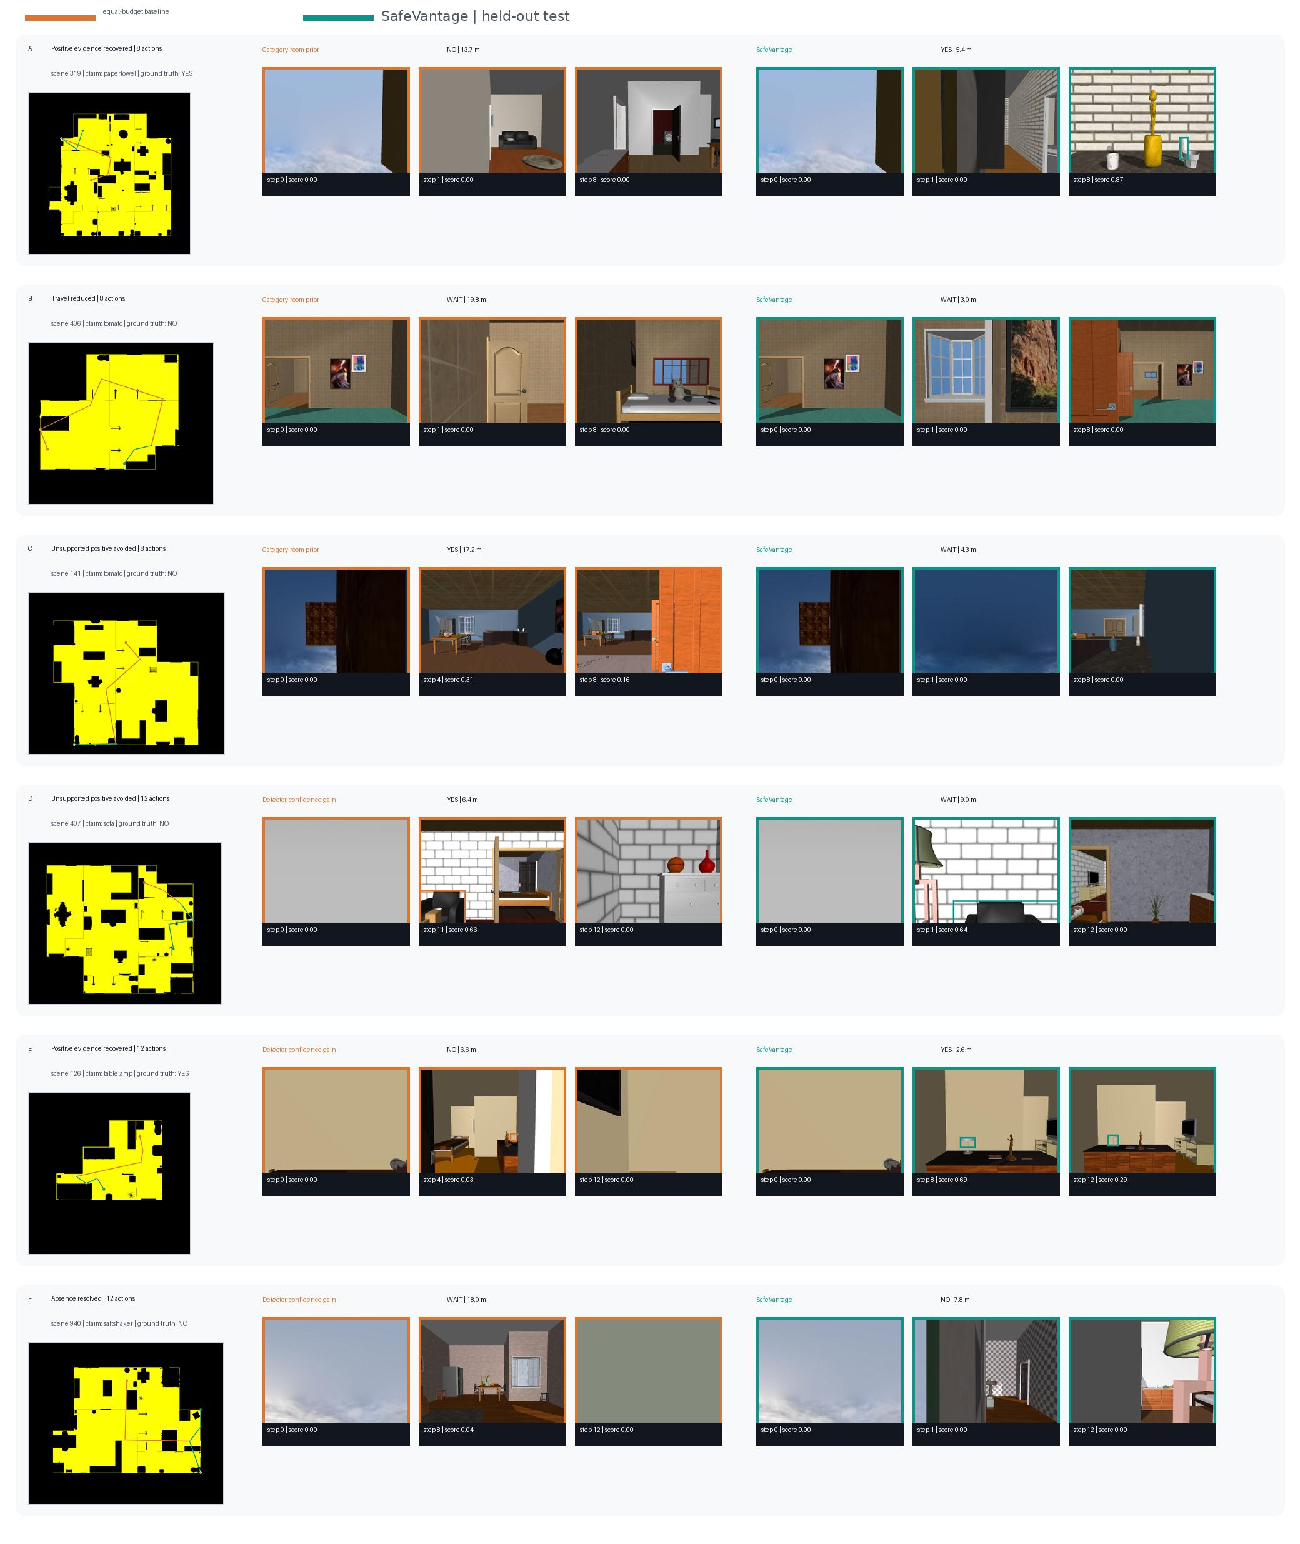
\includegraphics[width=\linewidth,height=0.84\textheight,keepaspectratio]{figures/fig_locked_trajectory_gallery.pdf}
%   \caption{\textbf{Six held-out acquisition-to-decision traces.} The gallery covers recovered evidence, avoided false positives, efficient \textsc{Wait}, and resolved absence at both action budgets.}
%   \label{fig:locked-gallery}
% \end{figure}
% \FloatBarrier

% \subsection{Category Breakdown}
% \label{app:category-diagnostics}
% Aggregate superiority need not be uniform across categories. Figure~\ref{fig:category-heatmap} compares \method{} with the primary baseline at each budget. Most category cells favor \method{}, and travel savings are broad at eight actions. The visible red cells are equally important: for example, twelve-action countertop macro-F1 is worse despite the aggregate win. These cells are descriptive slices with fewer episodes, not separately powered hypothesis tests.

% \begin{figure}[H]
%   \centering
%   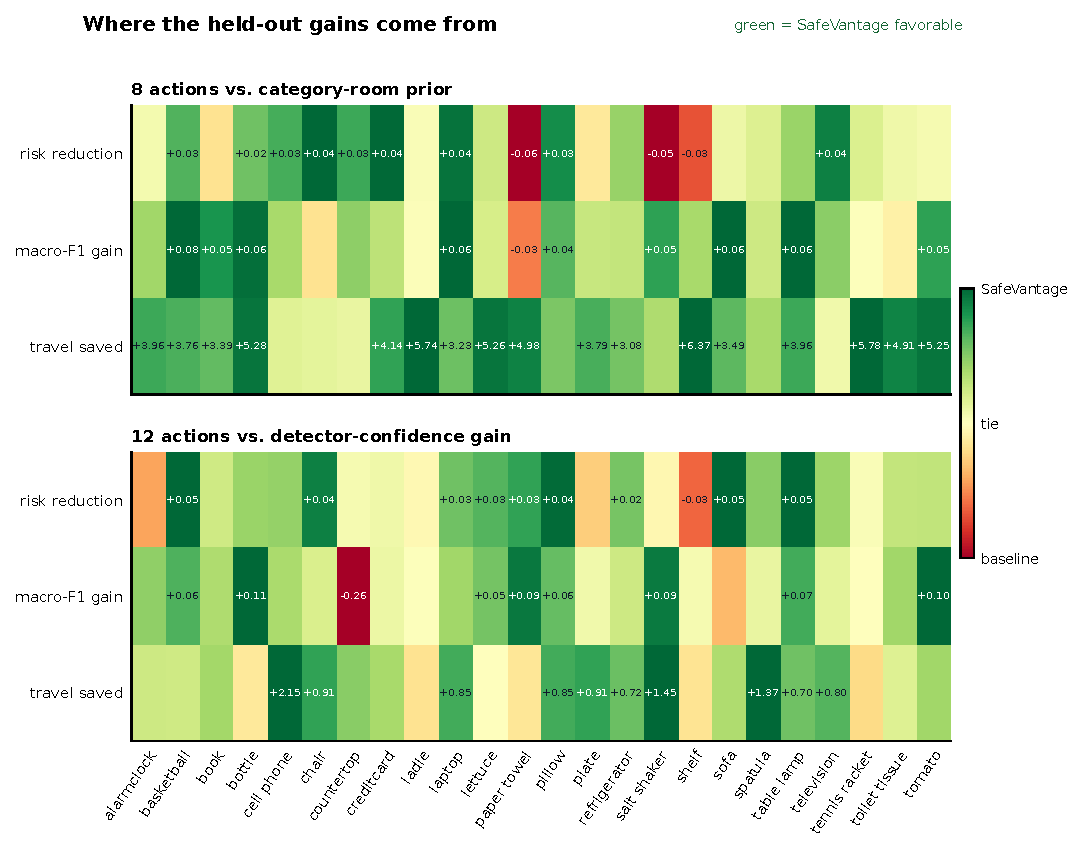
\includegraphics[width=\linewidth]{figures/fig_locked_category_heatmap.pdf}
%   \caption{\textbf{Category-level held-out effects.} Green favors \method{}; rows show risk reduction, macro-F1 gain, and travel saved at each budget.}
%   \label{fig:category-heatmap}
% \end{figure}

\section{Cross-Environment Evidence Studies}
\subsection{Equal-Input HM3D Operating Points}
Table~\ref{tab:main} reports the complete held-out HM3D ledger under one decision wrapper. All methods receive the same 160 RGB-D/pose frames.

\begin{table}[H]
  \centering
  \caption{\textbf{Equal-input HM3D operating points.} $R_9$ repeats calibration across nine folds; $R_{@\mathrm{cov}}$ matches coverage. Lower risk and AURC are better.}
  \label{tab:main}
  \resizebox{\linewidth}{!}{\begin{tabular}{lrrrrrrrr}
\toprule
method & cov. & acc. & FP & recall & risk & $R_{9}$ & $R_{@\mathrm{cov}}$ & AURC \\
\midrule
\textbf{SafeVantage} & 0.436 & \textbf{0.962} & \textbf{0.059} & 0.584 & \textbf{0.524} & \textbf{0.538} & \textbf{0.538} & \textbf{0.649} \\
Qwen2 caption-RAG & 0.565 & 0.881 & 0.240 & \textbf{0.692} & 0.715 & 0.638 & 0.685 & 0.715 \\
ConceptGraphs & 0.432 & 0.920 & 0.123 & 0.552 & 0.617 & 0.594 & 0.707 & 0.726 \\
VLMaps & 0.541 & 0.916 & 0.162 & 0.689 & 0.618 & 0.656 & 0.910 & 0.850 \\
\bottomrule
\end{tabular}
}
\end{table}

At the minimum-risk setting, \method{} reaches 0.436 coverage, 0.962 answered accuracy, 0.059 false-positive rate, and 0.524 risk. Its absolute risk reduction is 0.191 [0.130, 0.254] against caption-RAG, 0.094 [0.047, 0.142] against ConceptGraphs, and 0.099 [0.051, 0.148] against equal-view VLMaps. Across nine four-scene calibration folds, mean out-of-calibration risk is 0.538 for \method{}, 0.594 for ConceptGraphs, 0.638 for caption-RAG, and 0.656 for VLMaps; \method{} also has the lowest matched-coverage risk and AURC.

\subsection{ScanNet Supporting-View Intervention}
The ScanNet intervention keeps question, reader, prompt, rank, and history length fixed while changing only whether depth-verified target views occupy the selected ranks. Table~\ref{tab:causal} reports both readers and scene-clustered intervals against the target-absent condition.

\begin{table}[H]
  \centering
  \caption{\textbf{ScanNet supporting-view intervention.} Intervals compare each restored condition with target-absent histories.}
  \label{tab:causal}
  \begin{adjustbox}{max width=\columnwidth,max height=0.35\textheight}
    \begin{tabular}{llccc}
\toprule
reader & evidence set & F1 & $\Delta$ vs absent & scene CI \\
\midrule
Qwen2-VL & target absent & 0.2483 & -- & -- \\
Qwen2-VL & strongest 1 & 0.3565 & +0.1082 & [-0.0181, 0.2290] \\
Qwen2-VL & strongest 4 & 0.4410 & +0.1927 & [0.0691, 0.2977] \\
Qwen2-VL & complete & \textbf{0.4540} & \textbf{+0.2057} & \textbf{[0.0752, 0.3133]} \\
Qwen2.5-VL & target absent & 0.1888 & -- & -- \\
Qwen2.5-VL & complete & 0.3215 & +0.1327 & [0.0513, 0.2053] \\
\bottomrule
\end{tabular}


  \end{adjustbox}
\end{table}

% \subsection{HM3D Resolving-View Trace}
% \label{app:hm3dtraces}
% Figure~\ref{fig:active_trace} is the qualitative counterpart to the matched-cost selector result. Geometry and the 2D map choose 1.5-m actions that reveal zero queried-category pixels. The 3D evidence selector chooses a reachable 2.6-m geodesic action that reveals 419 vase pixels. Every candidate lies on the source navmesh component, and the mesh, path, rendered observation, semantic pixels, and decision ledger come from the same episode.

% \begin{figure}[H]
%   \centering
%   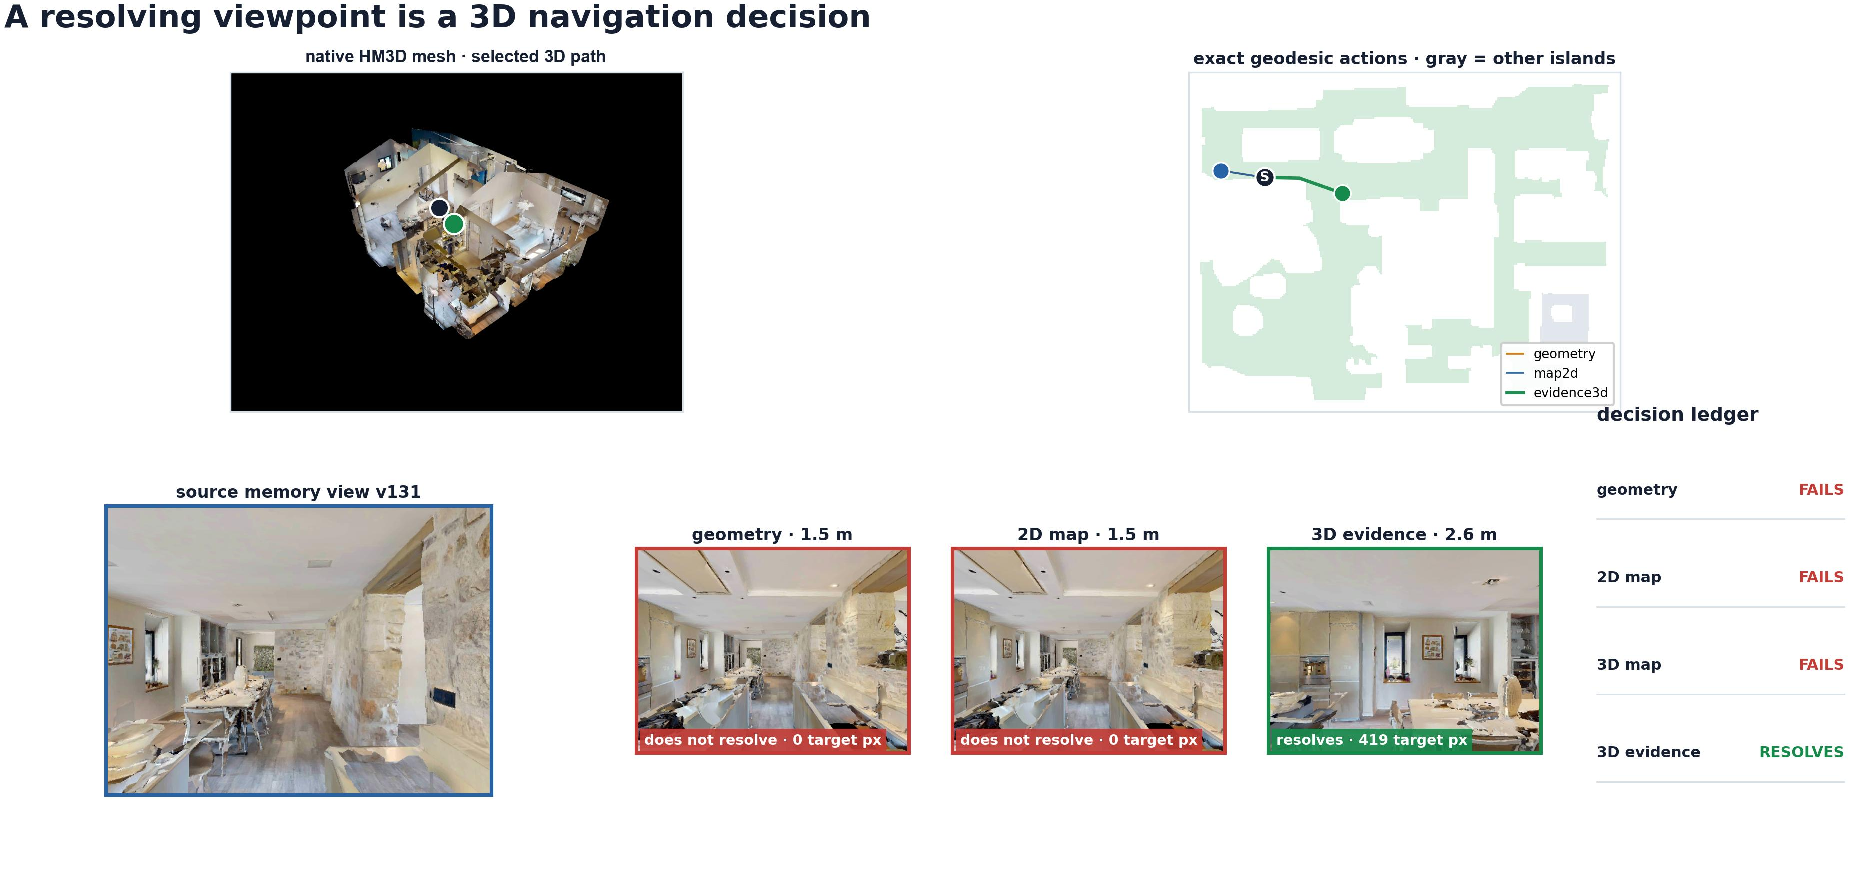
\includegraphics[width=\linewidth,height=0.84\textheight,keepaspectratio]{figures/fig50_hm3d_active_trace.pdf}
%   \caption{\textbf{An HM3D resolving-view trace.} Evidence-3D reveals 419 vase pixels from a reachable view missed by equal-budget geometry and 2D-map selectors.}
%   \label{fig:active_trace}
% \end{figure}
% \FloatBarrier

\section{Mechanism and Robustness}
% \subsection{Matched Component Audit}
% \label{app:component-audit}
% The component audit uses 116 ProcTHOR training scenes and 3,712 paired episodes per variant and budget. Each variant reruns acquisition, keeps the feature schema fixed, and refits the same selective-head architecture with scene-disjoint folds. The full-controller row reproduces the previously frozen training histories; row hashes are included in the artifact bundle.

% Table~\ref{tab:component-audit} gives the complete seven-variant ledger. Removing supporting-view identity or target-ray alignment lowers macro-F1 by 0.0565 at eight actions and about 0.0322 at twelve. Directed exploration is the long-horizon term: removing it lowers macro-F1 by 0.1345 and raises risk by 0.0373 at twelve actions. The confidence-backbone-only controller loses 0.0469/0.1615 macro-F1 at eight/twelve actions; yaw diversity and base geometry have smaller effects.

% \begin{table}[H]
%   \centering
%   \caption{\textbf{Train-OOF component audit.} Each removal reruns acquisition and refits the same scene-disjoint head on 116 scenes.}
%   \label{tab:component-audit}
%   \begin{adjustbox}{max width=\columnwidth,max height=0.35\textheight}
%   \scriptsize
%   \resizebox{\linewidth}{!}{\begin{tabular}{@{}lccc ccc@{}}
  \toprule
  & \multicolumn{3}{c}{8 actions} & \multicolumn{3}{c}{12 actions} \\
  \cmidrule(lr){2-4}\cmidrule(l){5-7}
  Variant & Risk$\downarrow$ & F1$\uparrow$ & Travel$\downarrow$ & Risk$\downarrow$ & F1$\uparrow$ & Travel$\downarrow$ \\
  \midrule
  \textbf{Full \method{}} & \textbf{0.3799} & \textbf{0.5712} & \textbf{2.89} & \textbf{0.3312} & \textbf{0.6736} & \textbf{6.29} \\
  $-$ claim provenance & 0.3940 & 0.5148 & 2.88 & 0.3510 & 0.6414 & 6.28 \\
  $-$ target-ray alignment & 0.3940 & 0.5148 & 2.88 & 0.3510 & 0.6413 & 6.28 \\
  $-$ yaw diversity & 0.3806 & 0.5706 & 2.90 & 0.3292 & 0.6744 & 6.29 \\
  $-$ base geometry & 0.3828 & 0.5617 & 3.05 & 0.3321 & 0.6714 & 6.29 \\
  $-$ directed exploration & 0.3847 & 0.5608 & 2.86 & 0.3685 & 0.5391 & 4.36 \\
  Confidence backbone only & 0.3892 & 0.5243 & 2.85 & 0.3808 & 0.5121 & 4.36 \\
  \bottomrule
\end{tabular}
}
%   \end{adjustbox}
% \end{table}

\subsection{Train-Frozen Validation Confirmation}
The seven variants are applied to 96 query-eligible validation houses with acquisition settings and train-fitted heads held fixed, yielding 3,072 paired episodes per row and budget. The full controller reaches macro-F1 0.5307/0.6149 at eight/twelve actions. Removing supporting-view identity loses 5.54/3.23 points; removing target-ray alignment loses 5.58/3.30. Directed exploration is the long-horizon term, losing 12.26 points at twelve actions, while the confidence backbone loses 13.14.

\begin{table}[H]
  \centering
  \caption{\textbf{Train-frozen component validation.} Loss is full-controller minus variant macro-F1 on 96 separate houses.}
  \label{tab:component-validation}
  \scriptsize
  \begin{adjustbox}{max width=\linewidth,max height=0.5\textheight}
    \begin{tabular*}{\columnwidth}{@{\extracolsep{\fill}}lcccc@{}}
  \toprule
  & \multicolumn{2}{c}{8 actions}
  & \multicolumn{2}{c}{12 actions} \\
  \cmidrule(lr){2-3}\cmidrule(l){4-5}

  Variant
  & F1$\uparrow$ & Loss (pp)$\downarrow$
  & F1$\uparrow$ & Loss (pp)$\downarrow$ \\
  \midrule

  \textbf{Full \method{}}
  & \textbf{0.5307} & --
  & \textbf{0.6149} & -- \\

  $-$ claim provenance
  & 0.4753 & \textbf{+5.54}
  & 0.5826 & \textbf{+3.23} \\

  $-$ target-ray alignment
  & 0.4749 & \textbf{+5.58}
  & 0.5819 & \textbf{+3.30} \\

  $-$ yaw diversity
  & 0.5311 & $-0.04$
  & 0.6162 & $-0.13$ \\

  $-$ base geometry
  & 0.5255 & \textbf{+0.52}
  & 0.6167 & $-0.18$ \\

  $-$ directed exploration
  & 0.5247 & \textbf{+0.60}
  & 0.4923 & \textbf{+12.26} \\

  \addlinespace[2pt]
  Confidence backbone only
  & 0.4847 & \textbf{+4.60}
  & 0.4835 & \textbf{+13.14} \\

  \bottomrule
\end{tabular*}
  \end{adjustbox}
\end{table}

% \begin{figure}[H]
%   \centering
%   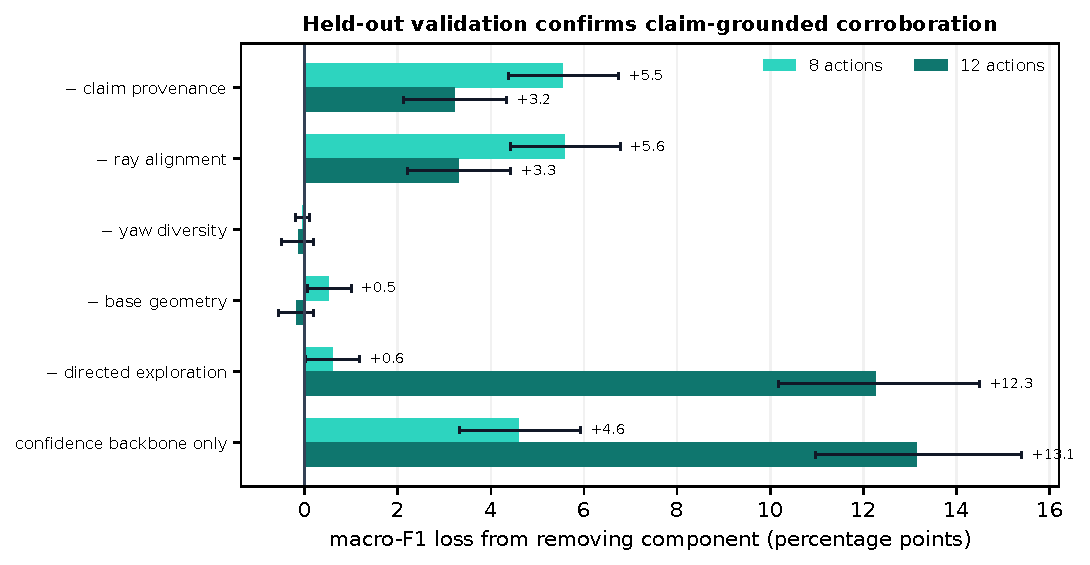
\includegraphics[width=\linewidth]{figures/fig_component_validation.pdf}
%   \caption{\textbf{Component effects transfer to validation.} Bars are macro-F1 losses from train-frozen removals; whiskers are paired 95\% scene-bootstrap intervals.}
%   \label{fig:component-validation}
% \end{figure}

\subsection{Robustness and Deployment Scope}
\label{app:robustness}
\textbf{Negative decisions.} Positive support and search coverage are complementary. A coverage measure uses the fraction of sampled view opportunities and source groups already observed, together with existing evidence scores. Its threshold is selected on six development scenes under a 5\% false-negative-decision constraint and evaluated on 12 held-out ScanNet scenes. It attains 0.983 observed-absent recall, 0.935 negative-decision precision, and 0.033 false decisions over non-absent states; a score-only low-confidence rule attains 0.051 absent recall and 0.500 precision.

\textbf{Correlated support.} Nearby frames can repeat the same observation. Pose clustering leaves the HM3D ranking stable in our control. In the active-policy audits, removing supporting-view identity or target-ray alignment lowers macro-F1 at both horizons in training OOF and train-frozen validation.

\textbf{Independent-view causal control.} The ten-case equal-count pilot is retained as a reader-side composition control. In the larger ScanNet study, answer quality changes as supporting views are removed and restored; the active-policy ablation separately measures their acquisition value.

\textbf{Acquisition--decision interface.} The HM3D traces separate whether a selector finds a resolving view from how a downstream wrapper uses it. The primary ProcTHOR experiment evaluates both stages end to end.

\textbf{Detector and action-graph dependence.} The ProcTHOR comparison uses fixed YOLO-World predictions on discrete viewpoints, so the policies differ in acquisition rather than detector outputs. Detector-shift controls and continuous robot execution are the next deployment tests.

\textbf{Cost sensitivity.} The headline risk uses $(C_{\mathrm{FP}},C_{\mathrm{FN}},C_{\mathrm{A}})=(5,2,0.5)$. We evaluate an 18-cell grid with false-positive costs $\{1,2,3,5,8,10\}$ and abstention costs $\{0.25,0.5,1\}$, refitting the two-threshold adapter on the same calibration scenes in every cell. At FP cost 5 and abstention cost 0.5, scene-macro risk favors \method{} over caption-RAG by 0.192 [0.129, 0.256], ConceptGraphs by 0.094 [0.047, 0.141], and equal-160-view VLMaps by 0.099 [0.052, 0.147]. At FP cost 10, the corresponding gains are 0.445 [0.324, 0.576], 0.185 [0.086, 0.280], and 0.251 [0.152, 0.352]. Across all cells, \method{} wins 12, 14, and 11 comparisons, respectively.

\clearpage
\input{checklist}

\end{document}
